% Exemplo de utilização da UFSCTeX.

\documentclass{ufsctex/ufsctex}

% Pacotes usados especificamente neste documento
\usepackage{tikz}
\usepackage{listings}
% The package listings is unable to deal correctly
% with multibyte strings.
% A workaround is to replace every "offending character"
% with its respective TeX escape codes.
%
% This is acomplished with the 'literate programming'
% feature of the listings package.
\lstset{
literate=
    {á}{{\' a}}1
    {Á}{{\' A}}1
    {à}{{\` a}}1
    {À}{{\` A}}1
    {â}{{\^ a}}1
    {Â}{{\^ A}}1
    {ã}{{\~ a}}1
    {Ã}{{\~ A}}1
    {ç}{{\c c}}1
    {Ç}{{\c C}}1
    {é}{{\' e}}1
    {É}{{\' E}}1
    {ê}{{\^ e}}1
    {Ê}{{\^ E}}1
    {í}{{\' \i}}1
    {Í}{{\' I}}1
    {ó}{{\' o}}1
    {Ó}{{\' O}}1
    {ô}{{\^ o}}1
    {Ô}{{\^ O}}1
    {õ}{{\~ o}}1
    {Õ}{{\~ O}}1
    {ú}{{\' u}}1
    {Ú}{{\' U}}1
}


\begin{document}

% Capa e folha de rosto

\instituicao[a]{Universidade Federal de Santa Catarina} % Opcional
\departamento[a]{DEPARTAMENTO DE INFORMÁTICA E ESTATÍSTICA}
\curso[o]{Curso de Sistemas de Informação}
\documento[o]{} % [o] para dissertação [a] para tese
\titulo{Proposta para desenvolvimento de um Data Warehouse}

\autor{Giancarlo Souza de Freitas, Ronan Romeu Knob, Sabrina Schütz de Oliveira, Valdir Luiz Hofer Arnhold}
\grau{aprovação parcial na disciplina de Data Warehouse}
\local{Florianópolis}
\data{04}{junho}{2017}
\orientador[Orientador]{Prof.  Jose Leomar Todesco, Dr.}


\capa
\folhaderosto[] % Se nao quiser imprimir a ficha, é só não usar o parâmetro

%% Informações sobre a banca

\numerodemembrosnabanca{4} % Isso decide se haverá uma folha adicional
\orientadornabanca{nao} % Se faz parte da banca definir como sim
\coorientadornabanca{sim} % Se faz parte da banca definir como sim
\bancaMembroA{Primeiro membro\\Universidade ...} %Nome do presidente da banca
\bancaMembroB{Segundo membro\\Universidade ...} % Nome do membro da Banca
\bancaMembroC{Terceiro membro\\Universidade ...} % Nome do membro da Banca
\bancaMembroD{Quarto membro\\Universidade ...} % Nome do membro da Banca
%\bancaMembroE{Quinto membro\\Universidade ...} % Nome do membro da Banca
%\bancaMembroF{Sexto membro\\Universidade ...} % Nome do membro da Banca
%\bancaMembroG{Sétimo membro\\Universidade ...} % Nome do membro da Banca

\folhaaprovacao

% % Dedicatória

\dedicatoria{
    Este trabalho é dedicado
    aos meus colegas de classe
    e aos meus queridos pais.
}

\paginadedicatoria

% % Agradecimentos

\agradecimento{
    Inserir os agradecimentos aos colaboradores
    à execução do trabalho.
}

\paginaagradecimento

% % Epígrafe

\epigrafe{
    Texto da Epígrafe.
    Citação relativa ao tema do trabalho.
    É opcional.
    A epígrafe pode também aparecer na abertura
    de cada seção ou capítulo.
}
{(Autor da epígrafe, ano)}

\paginaepigrafe

% % Resumo

\textoResumo{
    Um agente cognitivo artificial utiliza bases de conhecimentos sobre as quais faz inferências buscando tomar decisões. 
    Com o crescimento da produção de informação, gerando consequentemente conhecimento, é preciso que agentes inteligentes sejam capazes de armazenar e raciocinar sobre diferentes formas de conhecimento. 
    Além disso, a informação e o conhecimento são dinâmicos, dessa forma o agente também deve permitir que novas formas de representação de conhecimento sejam adicionadas ao seu ciclo de raciocínio. 
    Com essas premissas, o presente trabalho propõe a implementação de um interpretador para o desenvolvimento de agentes com base em sistemas multi-contexto para mapear o conhecimento. 
    Buscando possibilitar a integração de diferentes formas de conhecimento no ciclo de raciocínio. 
}
\palavrasChave{
    Agentes.
    Sistemas multi-contexto.
    Interpretador.
}

\paginaresumo

% % Resumo, em inglês.

\textAbstract{
    Resumo traduzido para outros idiomas,
    neste caso,
    inglês.
    Segue o formato do resumo
    feito na língua vernácula.
    As palavras-chave traduzidas,
    versão em língua estrangeira,
    são colocadas abaixo do texto
    precedidas pela expressão ``Keywords'',
    separadas por ponto.
}
\keywords{
    Keyword 1.
    Keyword 2.
    Keyword 3.
}

\paginaabstract

% Sumário e listas usadas no documento.
% As listas dependem da necessidade do usuário

\listadefiguras
\listadetabelas
%\listadeabreviaturas
%\listadesimbolos
\sumario


% Introdução

\chapter{Introdução}

\section{Contextualização}

A locadora Ronbuster, fundada em 1972, 
possui 4 filiais na grande florianópolis e, 
preocupada com o crescimento dos meios digitais 
de transmissão de filmes, decidiu implantar uma 
data mart para analisar o histórico de vendas, 
buscando novas estratégias para continuar 
crescendo no mercado.

O público da locadora é composto em sua maioria, 
por pessoas acima de 40 anos. Seu acervo é 
composto, em grande parte, por DVD’s e Blu-Rays. 
Também possui em acervo VHS, e outras mídias, 
mas em pequena quantidade.

As categorias de preço variam em função da data 
de chegada da mídia na locadora. Ao chegar na 
locadora, uma mídia é classificada como 
lançamento, e o empréstimo deve ser retornado 
em até 24 horas, por um preço de 8 reais. 
Depois de 60 dias do lançamento, a categoria 
da mídia muda para “vermelha”, e sua devolução 
pode ser feita em até 72 horas após o empréstimo, 
pelo valor de 6 reais. Passados 120 dias na 
categoria vermelha, a mídia passa para a 
categoria “verde” e o seu empréstimo pode ser 
devolvido em até 96 horas, com valor de 4 reais.
 
\section{Perguntas estratégicas}

As perguntas estratégias levantadas para o 
desenvolvimento do Data Mart são as seguintes:

\begin{enumerate}
    \item Em quanto tempo uma mídia física se paga?
    \item Qual é o fluxo de empréstimos e devoluções das mídias por dia da semana?    
    \begin{enumerate}
    \item Responde quais dias tem mais devolução e mais empréstimos.
    \end{enumerate}
    \item Qual o número ideal de cópias de cada título por filial?
    \end{enumerate}
  


\section{Escopo}

O escopo do projeto consiste em planejar e 
desenvolver um Data Mart para a locadora Ronbuster 
e suas filiais. De forma específica, para o 
desenvolvimento do mercado e a geração de receita.  
O número máximo de usuários suportados pelo sistema, 
para realizar a análise dos resultados gerados pelo 
\textit{Data Mart} é de 10 pessoas. 


\section{Justificativa}

A gestão da informação, quando feita de forma correta, pode trazer inúmeros benefícios para as organizações. Com a implantação do Data Mart na locadora Ronbuster, se busca aumentar o lucro sobre as locações de mídias do acervo, gerando um maior fluxo de caixa para empresa. Além do mais, numa sociedade que cresce em competitividade a cada dia, um data mart pode ser um diferencial no mercado para responder rapidamente às demandas e tendências do mercado.

Para estimar o retorno do projeto, em um período anual, 
foi utilizado a técnica simples do 
\textit{Payback Period Analysis}, onde foi feita uma 
estimativa do retorno estimado ao ano de 
impacto nas vendas, e diluído o valor do 
projeto em parcelas deste retorno anual, 
conforme é mostrado na Tabela \ref{tab:justificativa}.

\begin{table}[!htb]
    \begin{center}
        \caption{\textit{Payback Period Analysis}.} \label{tab:justificativa}
        \begin{tabular}{ p{6cm} | p{3cm} }
            \hline
            \textbf{Custo estimado do projeto do Ronbuster \textit{Data Mart}} & R\$ 52.000,00 \\
            \hline
            \textbf{Custo do retorno anual} & R\$ 37.000,00 \\
            \hline
            \textbf{\textit{Payback Period Analysis}} & 1,4 anos \\
            \hline
        \end{tabular}
    \end{center}
    Fonte: Os autores (2017).
\end{table}

Como visto na tabela acima, com a implantação do data mart 
na rede de locadoras Ronbuster foi calculado uma receita 
a mais de R\$13.500,00 para a empresa a cada ano. 
Isso é, após 2,6 anos, que é o período de 
Payback, a empresa lucrará 13,45\% a mais, 
anualmente, pelo uso da ferramenta, considerando o 
levantamento de R\$ 275.000,00 aproximadamente de 
receita das filiais da locadora juntas, anualmente.

Além do próprio projeto se pagar num tempo aceitável, 
o valor das informações sobre o negócio, mesmo que 
não mensurados e usados no cálculo, devem ser levados 
em conta. Sendo assim, o projeto de instalação do 
data mart se torna viável e traz um bom retorno 
em médio prazo para a empresa.

\section{Fatores críticos de sucesso}

Os fatores críticos de sucesso, inicialmente 
levantados, são os seguintes:

\begin{itemize}
    \item Prover uma fonte única de informações sobre os processos de negócio da vídeo locadora.
    \item Aumentar a eficácia das locações, em 25\% ,  nos períodos de promoções.
\end{itemize}

\section{Exclusões de escopo}

Nesta etapa de desenvolvimento não será feita uma integração de dados com sistemas de terceiros.  Além disso, na primeira versão do projeto não vai ser disponibilizado ferramentas para descoberta de dados utilizando data mining.


\section{Riscos}

Os possíveis riscos levantados e seu plano de resposta e mitigação são
apresentados na Tabela \ref{tab:riscos}. 

\begin{table}[!htb]
    \begin{center}
        \caption{Riscos.} \label{tab:riscos}
        \begin{tabular}{ p{1.7cm} | p{2cm} | p{1.1cm} | p{2cm} | p{2cm} }
            \hline
            \textbf{Risco} &\textbf{Probabilidade} &\textbf{Impacto} & \textbf{Estratégia de resposta} & \textbf{Estratégia de mitigação} \\
            \hline
            Alteração do
            escopo
             &  Alta  &  Alto  &  Redefinição
             do tempo
               & Validação dos requisitos iniciais  \\
            \hline
            Dificuldade técnica &  Média  &  Alto  &  Contratação de especialista  &  Capacitação técnica para a equipe  \\
            \hline
        \end{tabular}
    \end{center}
    Fonte: Os autores (2017).
\end{table}
 


% Desenvolvimento

\chapter{Planejamento}

\section{Definição da equipe}

Os recursos humanos e seus respectivos papéis 
envolvidos no projeto são definidos na Tabela \ref{tab:recursos} . 

\begin{table}[!htb]
    \begin{center}
        \caption{Recursos Humanos.} \label{tab:recursos}
        \begin{tabular}{ p{4cm} | p{4cm} }
            \hline
            \textbf{Papel} & \textbf{Recurso Humano} \\
            \hline
            Diretor de DW & Ronan Romeu Knob \\
            \hline
            Gerente de projetos de DW & Sabrina Schütz de Oliveira
             \\
            \hline
            Analista de negócios & Giancarlo Souza de Freitas \\
            \hline
            Arquiteto de DW & Giancarlo Souza de Freitas \\
            \hline
            Equipe técnica & Valdir Luiz Hofer Arnhold \\
            \hline
        \end{tabular}
    \end{center}
    Fonte: Os autores (2017).
\end{table}
 
\section{Cronograma}

O projeto de \textit{Data Mart} Ronbuster 
foi pensado para ter início no mês 
de março. Sua duração estimada foi 
estipulada em 6 meses, contemplando as 
fases apresentadas no tabela x. 
A escolha deste período de início foi 
devido a que é o período de término das 
férias escolares, o que deve baixar o movimento 
das filiais, estando pronto também antes do final 
do ano, novo grande ciclo de férias.

Sendo assim, as datas iniciais de início e término do projeto são:

\begin{itemize}
    \item Início do projeto - 01/03/2017;    
    \item Término do projeto - 31/08/2017;    
    \item Dias úteis neste período: 129; e
    \item Horas do projeto: 1032h
\end{itemize}

Abaixo temos uma estimativa das fases do projeto, e seu tempo esperado.
Os valores apresentados não consideram feriados e sábados e domingos. Cálculo da hora é feito por dias úteis * 8h.

\begin{table}[!htb]
    \begin{center}
        \caption{Estimativa de tempo.} \label{tab:tempo}
        \begin{tabular}{ p{3cm} |  p{2.2cm} | p{2.3cm} | p{1.2cm} }
            \hline
            \textbf{Fase} & \textbf{Data de início}  & \textbf{Data de término} & \textbf{Duração} \\
            \hline
            Planejamento do projeto & 01/03/2017 & 24/03/2017 & 144 h \\
            \hline
            Entrevistas &
            27/03/2017 &
            07/04/2017 &
            80 h \\
            \hline
            Definição do esquema estrela e plano de ação &
            10/04/2017 &
            20/04/2017 &
            64 h \\
            \hline        
            Definição da equipe do DW &
            24/04/2017 &
            26/04/2017 &
            24 h \\
            \hline 
            Implementação do DW &
            27/04/2017 &
            09/06/2017 &
            248 h \\
            \hline            
            Criação de portal de dashboards e relatórios &
            12/06/2017 &
            04/08/2017 &
            320 h \\
            \hline 
            Treinamento &
            07/08/2017 &
            11/08/2017 &
            40 h \\
            \hline
            Homologação e ajustes pontuais &
            14/08/2017 &
            31/08/2017 &
            112 h \\
            \hline
            \multicolumn{3}{r|}{Total} & 1032 h \\
            \hline

        \end{tabular}
    \end{center}
    Fonte: Os autores (2017).
\end{table}


\section{Custos}

Com base no Cronograma mostrado e nas horas estimadas o custo projeto é de R\$ 52.000,00.

\chapter{MODELAGEM DIMENSIONAL}

Para a construção do modelo dimensional, 4 passos são necessários, sendo eles:

\begin{enumerate}
\item Decisão de qual processo de negócio deve-se modelar, com base na combinação do conhecimento do negócio com o conhecimento dos dados disponíveis.
\item Definição do grão do processo do negócio, o qual é o nível fundamental atômico de dados que representará o processo na tabela de fatos.
\item Escolha das dimensões que serão aplicadas a cada registro da tabela de fatos.
\item Escolha dos fatos mensuráveis que irão popular cada registro da tabela de fatos.
\end{enumerate}

A seguir, temos a utilização desses passos para a criação da modelagem dimensional em questão, para auxiliar a resolução das perguntas estratégicas levantadas.
 
\section{processo do negócio}

O processo do negócio que será modelado é o movimento diário de item, nos permitindo acompanhar quais filmes estão sendo emprestados, em que lojas, a que preço e em que dias.


\section{Granularidade}

A granularidade, representa o nível de
detalhamento da modelagem.
Para este projeto, se buscou alcançar o maior nível de granularidade possível. Por exemplo, para o 
mapeamento da dimensão do tempo é utilizado a hora, 
dessa forma se torna possível fazer 
consultas por dia ou semanas. 

\section{Dimensões}

As dimensões escolhidas são Tempo, Midia e Loja , conforme mostra a Figura \ref{fig:dimensoes}.  

\begin{figure}[!htb]
   \centering
   \caption{Dimensões.}\label{fig:dimensoes} 
   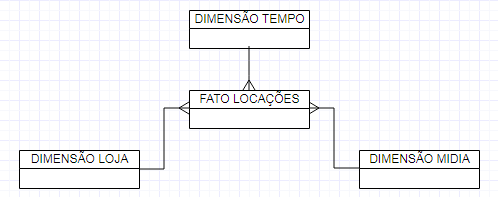
\includegraphics[scale=0.7]{imagens/img1.png}
\end{figure}

\section{Fatos}

Inicialmente foi modelada a seguinte a tabela de fatos de Locações, conforme mostra a Figura \ref{fig:fato0}.


\begin{figure}[!htb]
   \centering
   \caption{Fato - Versão 1.}\label{fig:fato0} 
   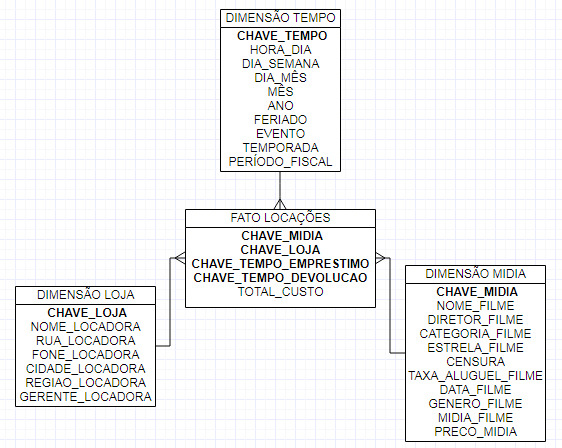
\includegraphics[scale=0.5]{imagens/fato-0.jpeg}
\end{figure}

"Há somente uma garantia para qualquer projeto de DW 
e é a que ele será mudado.” Depois de analisarmos 
novamente a modelagem, e com as perguntas estratégicas 
em mente, percebemos que uma nova tabela fato deveria ser 
adicionada para a resolução dessas perguntas, conforme é mostrado na Figura
 \ref{fig:fato}. 

\begin{figure}[!htb]
   \centering
   \caption{Fato - Versão 2.}\label{fig:fato} 
   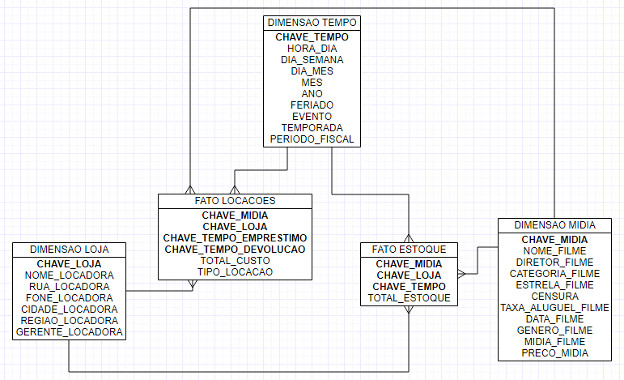
\includegraphics[scale=0.5]{imagens/fato-1.jpeg}
\end{figure}

 
\chapter{Indicadores}

Para verificar se as perguntas estratégicas 
levantadas no projeto da locadora Ronbuster 
estão sendo respondidas, é necessário criar indicadores. 
Os indicadores visam monitorar as variáveis necessárias para 
solucionar uma pergunta estratégica, e criando informação a partir 
delas, que responde aos questionamentos da gestão da empresa. 
Os indicadores são chamados indicadores estratégicos, que são os 
indicadores que podem dar ampla visão dos objetivos e metas mais 
gerais da empresa, bem como permitir a comparação de ações anteriores 
com resultados atuais. 

Quanto a locadora Ronbuster, para responder as perguntas que criamos, 
foram levantados os indicadores mostrados na Tabela \ref{tab:indi} e as 
variáveis mostradas na Tabela \ref{tab:variaveis}.

\begin{table}[!htb]
    \begin{center}
        \caption{Indicadores.} \label{tab:indi}
        \begin{tabular}{ p{4.5cm} |  p{4.5cm}   }
            \hline
            \textbf{Pergunta} & \textbf{Indicador}   \\
            \hline
            Em quanto tempo uma mídia física se paga? & (V1*v4) / (V2*V3) \\
            \hline
            Qual é o fluxo de empréstimos e devoluções das mídias por dia da semana? & (V5*24) e (V5*24)  \\
            \hline
           Qual o número ideal de cópias de cada título por filial? & V7 \\
            \hline

        \end{tabular}
    \end{center}
    Fonte: Os autores (2017).
\end{table}


\begin{table}[!htb]
    \begin{center}
        \caption{Variáveis.} \label{tab:variaveis}
        \begin{tabular}{ p{8cm}    }
            \hline
              V1 - Valor da locação de uma mídia \\
            \hline
              V2 - Custo da mídia (custo de compra de uma unidade) \\
            \hline
            V3 - Quantidade de mídias compradas   \\
            \hline
           V4 - Número de locações de uma mídia \\
            \hline
             V5 - Número de locações por hora \\
            \hline
             V6 - Número de devoluções por hora \\
            \hline
            V7 - Número de títulos disponíveis por hora do título \\
        \hline
        \end{tabular}
    \end{center}
    Fonte: Os autores (2017).
\end{table}

\section{Exemplos de relatórios}

\subsection{Pergunta 1}

A consulta para responder a pergunta 1, 
pode ser como acima. Nela, é apresentado o 
título da mídia, preço desta. Para resolver 
quanto tempo, foi calculado a média do custo da locação, 
considerando que pode haver diferença de custo por algum motivo, 
dividido pela média de dias que ela esteve locada. Considerando 
então uma locação de 24h, ou seja,1 locação por dia, temos, dividindo 
o preço por esta média, o número de dias em que a mídia se pagará.

\begin{figure}[!htb]
   \centering
   \caption{Resposta da pergunta 1.}\label{fig:fato} 
   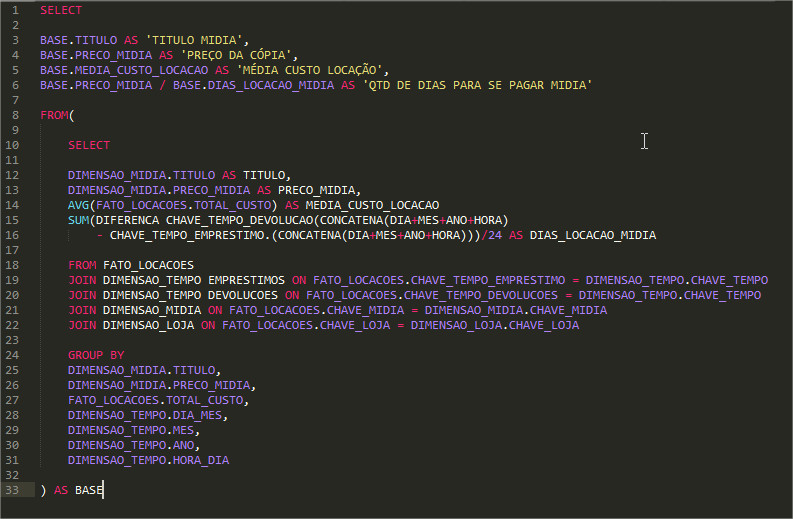
\includegraphics[scale=0.4]{imagens/sql-1.jpeg}
\end{figure}

As funções de diferença de tempo e concatenação de 
campos para formar as datas foram omitidas por apresentarem 
peculiaridades técnicas pertencentes a cada SGBD.

\subsection{Pergunta 2}

Para a pergunta estratégica 2: Qual é o fluxo de empréstimos e devoluções das mídias por dia da semana?

\begin{figure}[!htb]
   \centering
   \caption{Resposta da pergunta 2.}\label{fig:fato} 
   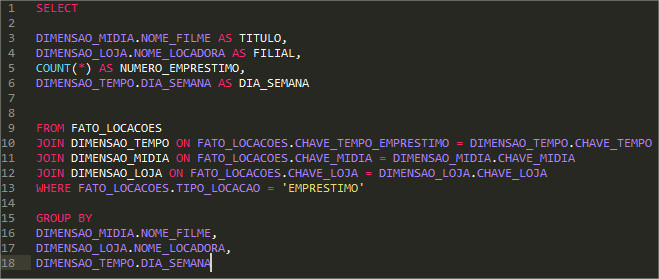
\includegraphics[scale=0.5]{imagens/sql-0.jpeg}
\end{figure}

Essa pesquisa retorna os dias da semana e a quantidade 
de cópias emprestadas, separados por título  e filial. 
A agregação poderia ser por qualquer unidade de tempo. 
Para saber a quantidade de devoluções, como a pergunta 2 
também exige, precisaria apenas mudar, na linha 13, a palavra 
\textbf{'EMPRESTIMO'} para \textbf{'DEVOLUCAO'}, e a chave da tabela 
de \textbf{'FATO\_LOCACOES'} para 
\textbf{'CHAVE\_TEMPO\_DEVOLUCAO'} .

 % Aqui vêm uma sequência de capítulos
% % Conclusão

\chapter{CONCLUSÃO}

De forma geral, conforme mostrado nas seções anteriores, com a modelagem dimensional, os indicadores criados e os modelos de consulta, é possível responder as perguntas estratégicas elaboradas. Com isso, se esperar aumentar a rentabilidade da organização através de uma fonte única de dados, organizados com qualidade. 


%\bibliographystyle{abnt-alf}
%\bibliography{bibliografia}

%\apendice
%\input{apendices/exemplo}
% O comando \apendice deve aparecer apenas uma vez,
% antes de todos os apêndices.

%\anexo
%\input{anexos/exemplo}
% O comando \anexo também deve aparecer apenas uma vez.

\end{document}
